\documentclass[../main.tex]{subfiles}

% 2.2.1 Extinktion
% 2.2.1.1 Was ist es?
Die Extinktion $E$ beschreibt die Abschwächung einer Welle nach der Durchquerung einer Substanz. In der Abschwächung spielen Absorption, Streuung, Beugung und Reflexion (Abb. \ref{fig:extinktion_typen}) eine Rolle.

% TODO alternative image (copyright..)
\begin{figure}[ht]
    \centering
    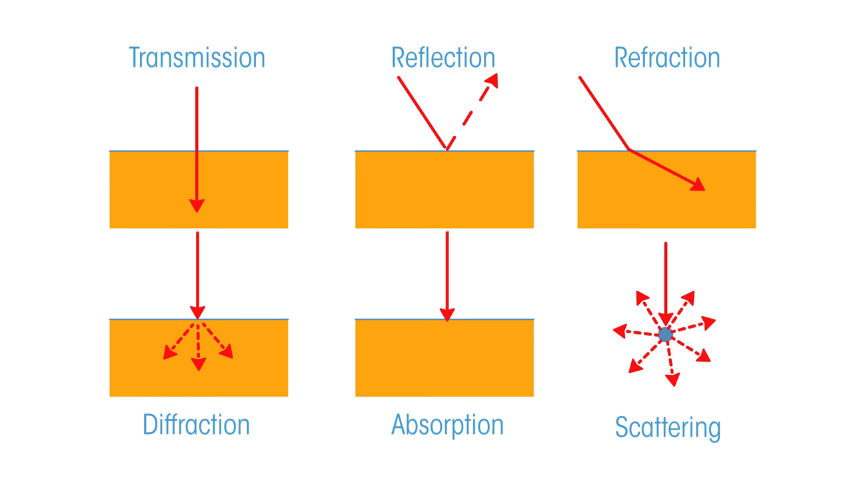
\includegraphics[width=0.65\textwidth]{extinktion_typen.png}
    \caption{Einflussfaktoren auf Extinktion}
    \label{fig:extinktion_typen}
\end{figure}

% 2.2.2 Absorption
Absorption beschreibt in der Physik die Aufnahme von Wellen in einer Substanz.

% 2.2.3 Streuung
Streuung ist die Ablenkung von Wellen in mehrere Richtungen.

% 2.2.4 Beugung
Wenn Strahlungen eine Substanz mit unterschiedlicher Dichte durchqueren, kommt es zu einer Verlangsamung der Ausbreitung, und damit zu einer Richtungsänderung. Das ist Beugung.

% 2.2.5 Reflexion
Glatte Oberflächen reflektieren häufig Strahlungen (z.B. Spiegel).